\documentclass[conference]{IEEEtran}
\IEEEoverridecommandlockouts
% The preceding line is only needed to identify funding in the first footnote. If that is unneeded, please comment it out.
\usepackage{cite}
\usepackage{amsmath,amssymb,amsfonts}
\usepackage{algorithmic}
\usepackage{graphicx}
\usepackage{textcomp}
\usepackage{xcolor}
\graphicspath{{figs/}{report/figs/}}
\def\BibTeX{{\rm B\kern-.05em{\sc i\kern-.025em b}\kern-.08em
    T\kern-.1667em\lower.7ex\hbox{E}\kern-.125emX}}
\begin{document}

\title{Impact of Network Topology on Distributed Inference:\\
Circulant Graphs as a Drop-In Replacement for 3D Torus Interconnects}

\author{
\IEEEauthorblockN{Nikhil Vemuri}
\IEEEauthorblockA{nvemuri@mit.edu}
\and
\IEEEauthorblockN{Brian Zhang}
\IEEEauthorblockA{zhangbr@mit.edu}
}

\maketitle

% NOTE: 4-page limit, not including references and the ``LLM Usage'' section.
% 5 pages are allowed for the graduate version of the class.

\section{Introduction}
Modern large-model inference is no longer a single-accelerator problem. Serving
large dense models and mixture-of-experts (MoE) layers
requires distributing tensors across many accelerator chips, which turns the
inter-chip network into a first-order performance constraint. Google's TPU v4
systems use a 3D torus with six inter-chip interconnect links per chip, but the
reason this topology is a good fit for inference communication is not obvious:
the best topology depends on which collective operations the mapper induces, how
those collectives load physical links, and whether the mapping itself changes
once realistic network costs are included.

This project studies the impact of network topology on distributed inference by
coupling AccelForge's mapping flow with a topology-aware interconnect model. We
model a 64-chip TPU-v4-like system and compare rings, meshes, tori, and
circulant graphs under comparable hardware budgets. The mapper first selects a
spatial partitioning using a logical
\texttt{NetworkMemory} level. We then extract the resulting inter-chip tensor
traffic, infer collective operations such as AllReduce, ReduceScatter,
AllGather, Broadcast, and point-to-point transfers, and replay those transfers
on candidate physical topologies using link-level bottleneck costs. The measured
network costs are fed back into the mapper until the proxy costs stabilize.

\begin{figure}[!t]
\centering
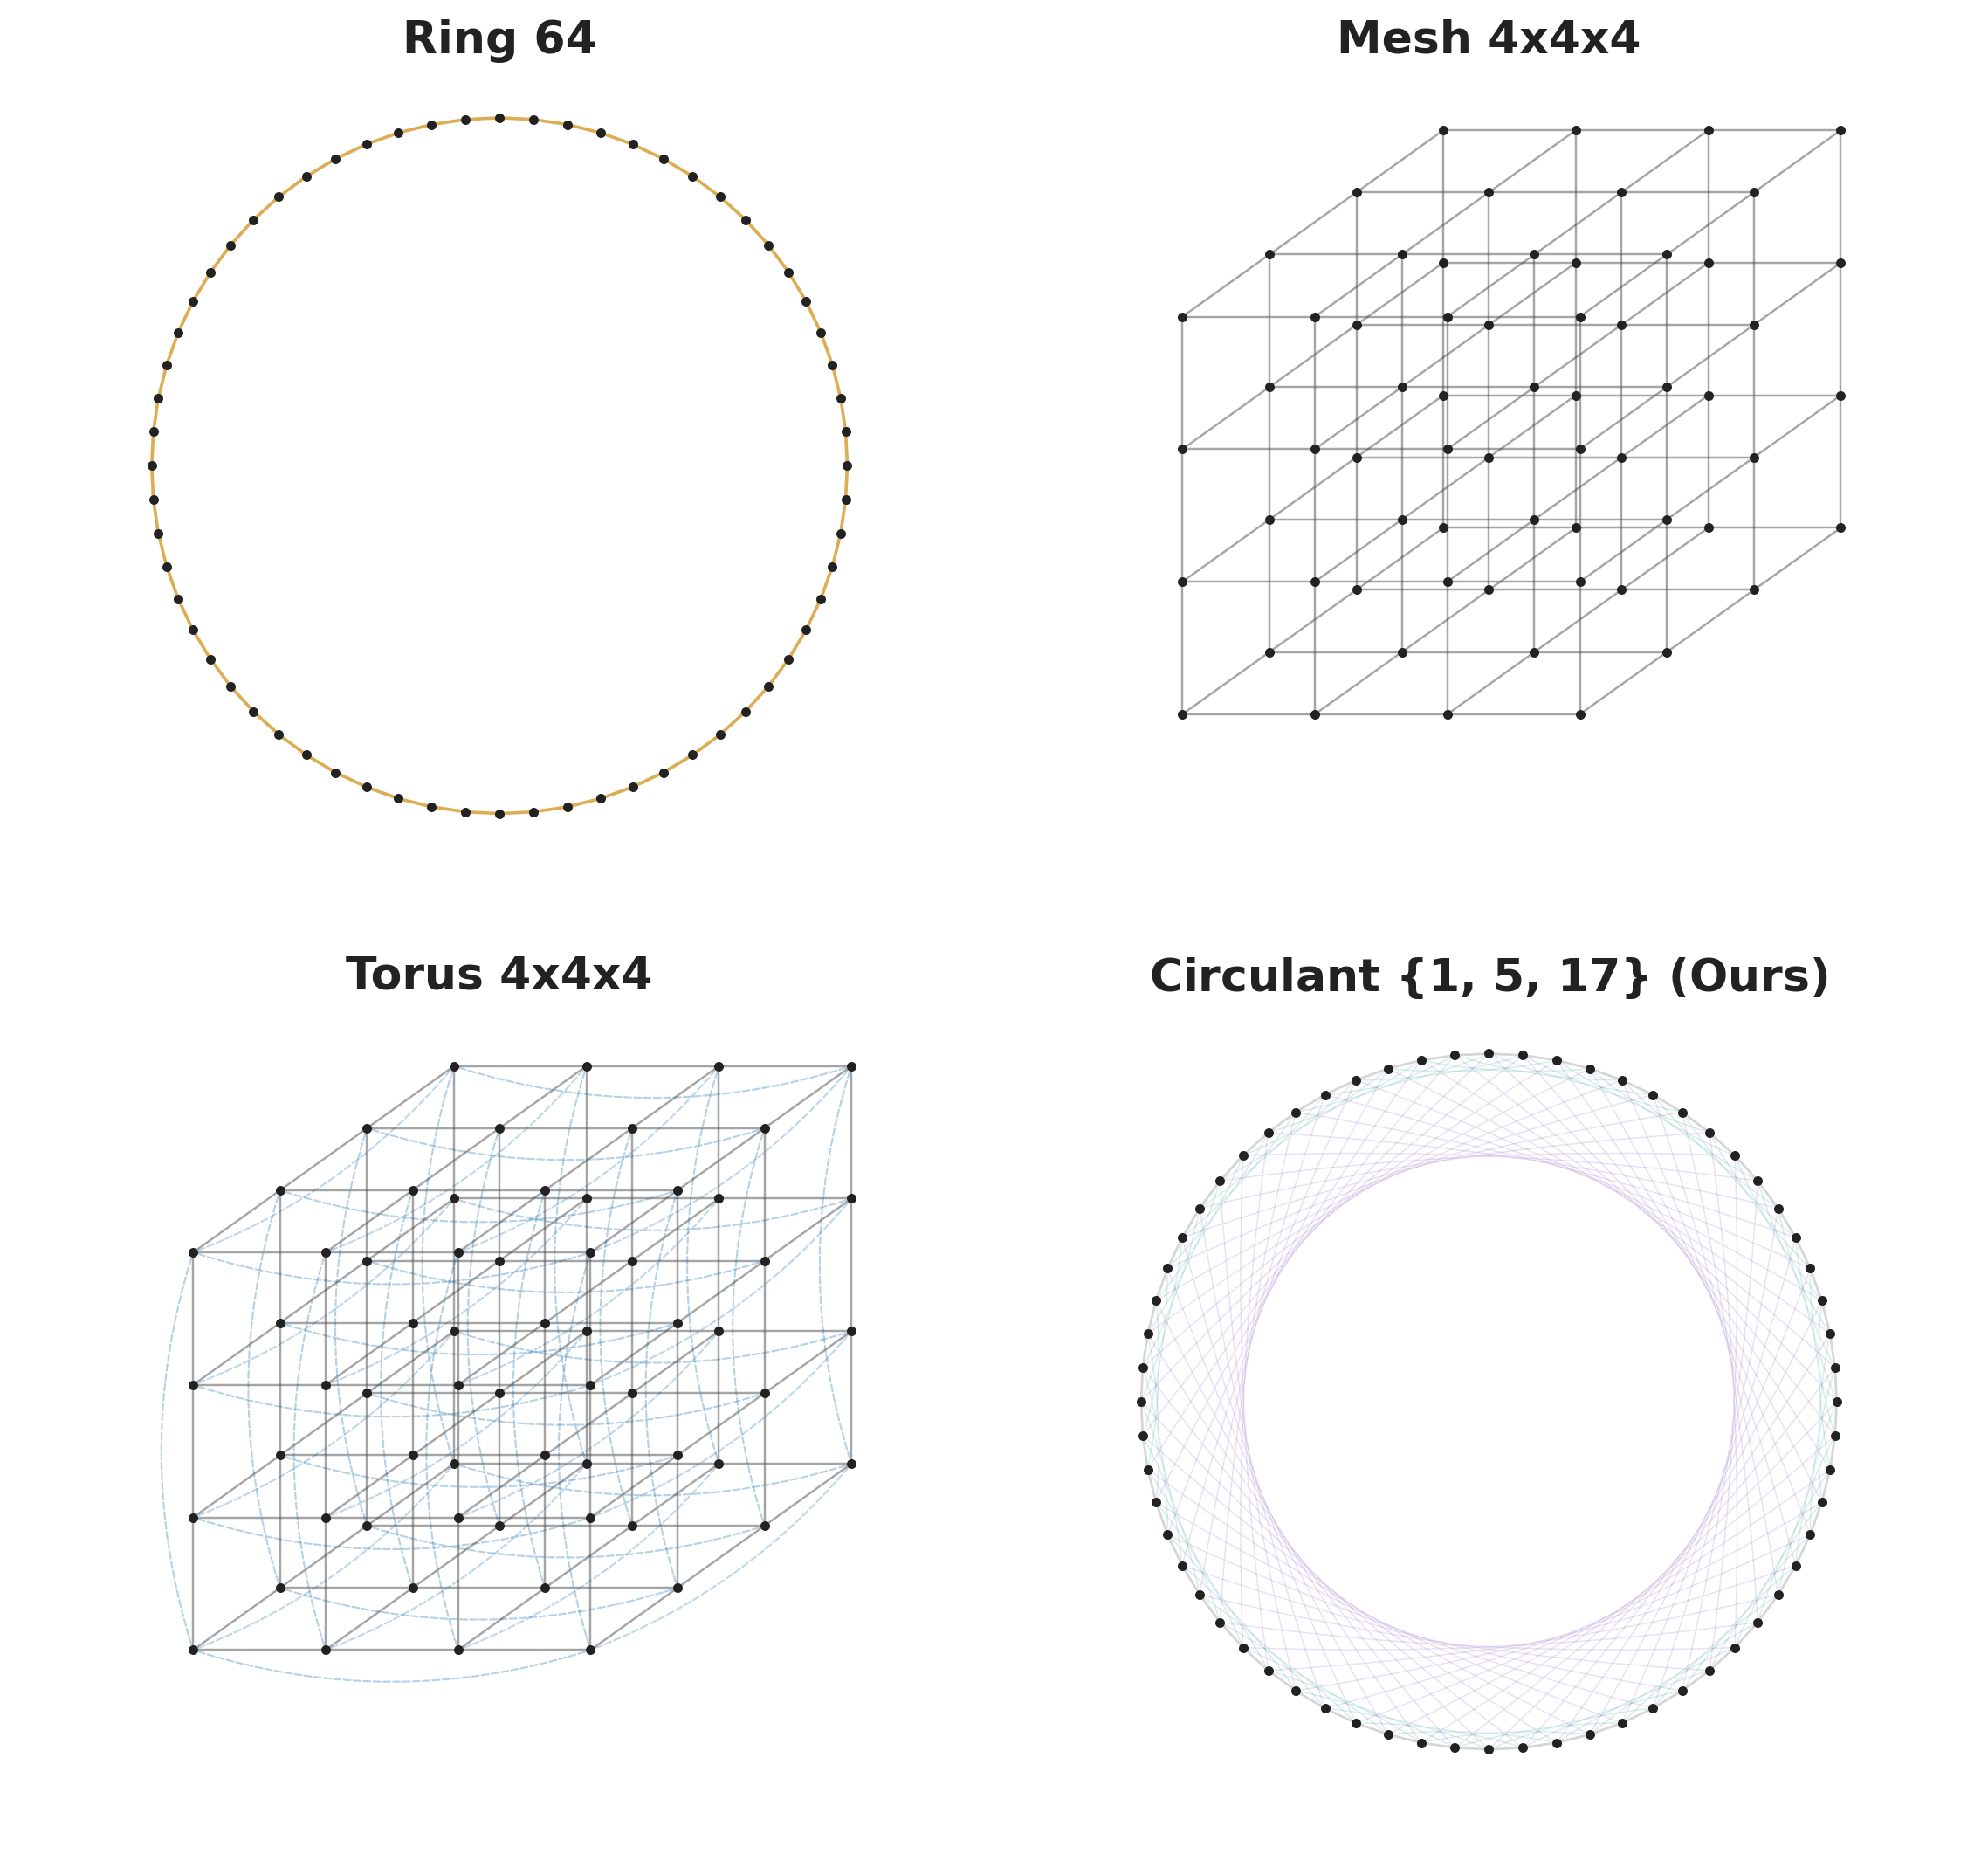
\includegraphics[width=0.92\linewidth]{topology_schematics.png}
\caption{The four 64-chip network topologies evaluated in the main study:
ring, 3D mesh, 3D torus, and the proposed circulant graph.}
\label{fig:topology-schematics}
\end{figure}

Our main proposal is the circulant graph $C(64,\{1,5,17\})$. We compare it to
three other topologies on the same number of chips (64): ring, 3D torus, and 3D
mesh. Figure~\ref{fig:topology-schematics} shows the topology schematics. We
motivate the circulant topology as a drop-in
replacement for a 64-chip 3D torus with the same six-link-per-chip budget. Each
generator forms an edge-disjoint Hamiltonian cycle, allowing AllReduce traffic
to be split across three full-chip rings with no shared directed links. This
structure reduces the AllReduce bottleneck-link load by $2.29\times$ relative
to the 3D torus's dimension-wise ring schedule, while also reducing graph
diameter from 6 to 4 hops.

We evaluate this design across small batched matrix multiplications, tall
matrix multiplications that resemble long-context attention projections,
square attention-like matrix multiplications, and MoE expert-FFN workloads.
Three findings emerge. First, topology choice alone causes multi-fold latency
differences: the circulant graph wins all 38 evaluated small, tall, and square
matmul cases and all four mapper-backed MoE cases. Second, the benefit comes
from bottleneck-link load rather than first-byte latency; serialization
dominates at the message sizes generated by these workloads. Third,
topology-aware feedback changes the estimated network cost substantially but has
low mapping sensitivity in our evaluated runs: the feedback loop converges in
two iterations and the inferred collective plan is stable from the first to
final mapping.


\section{Related Work}
TPU v4 motivates our baseline because it uses a 3D torus-style inter-chip
interconnect for large accelerator pods \cite{tpuv4}. Prior distributed deep
learning systems show that transformer inference and training rely heavily on
collectives such as AllReduce, especially under tensor parallelism
\cite{megatron}. MoE models add sparse all-to-all token dispatch and combine
traffic \cite{gshard,switch}. Circulant and multi-loop networks have also been
studied as low-degree interconnection networks \cite{circulant_survey}; our
work differs by evaluating such graphs inside an accelerator mapping loop
rather than only as abstract graph families.

\section{Design}
\subsection{Topology Cost Model}
The network model represents each topology as a graph with TPU-v4-like links:
45 GB/s unidirectional bandwidth, 4 pJ/bit/hop energy, and 500 ns per hop. A
transfer is routed onto directed physical links. Energy is the total bit-hop
cost,
\begin{equation}
E = 8 \alpha \sum_{\ell} B_{\ell},
\end{equation}
where $B_{\ell}$ is the byte load on link $\ell$ and $\alpha$ is the
energy-per-bit-per-hop. Latency is the bottleneck serialization time plus a
first-byte hop term,
\begin{equation}
L = \max_{\ell} B_{\ell}/\beta + D\lambda,
\end{equation}
where $\beta$ is link bandwidth, $D$ is graph diameter, and $\lambda$ is
per-hop latency. For the mapper-backed matmul and MoE expert-FFN experiments,
collectives are costed independently and summed in workload order. Sparse MoE
dispatch/combine replays in the repository merge all point-to-point transfers
inside one phase before costing because those sends are logically concurrent.

Topology-specific routing is important. Rings use the standard ring AllReduce.
Tori use independent per-dimension ring collectives. Meshes use linear
pipelines because they do not have wraparound links. Generic graphs fall back to
shortest paths, while the proposed circulant graph uses its Hamiltonian cycles
for full-chip AllReduce.

\subsection{AccelForge Feedback Loop}
AccelForge maps a workload onto a chip hierarchy whose outer level is a logical
\texttt{NetworkMemory}. That level initially has HBM-like per-byte proxy costs.
After mapping, we read the mapper's \texttt{NetworkMemory} accesses, identify
which tensor ranks were sharded across chips, infer the required collective, and
evaluate that collective on the physical topology. The resulting per-byte read
and write costs are fed back into \texttt{NetworkMemory}. This repeats until the
largest proxy change is below 5\% or six iterations are reached. In the
evaluated runs, every successful topology/workload pair converged in two
iterations.

\subsection{Circulant Topology}
The proposed topology is $C(64,\{1,5,17\})$: chip $i$ connects to
$(i \pm g) \bmod 64$ for each generator $g$. Since all three generators are
coprime to 64, each generator forms a Hamiltonian cycle over all chips. These
cycles are edge-disjoint, so AllReduce splits data into three chunks and runs
three ring AllReduces in parallel. For message size $B$, each circulant
directed link carries
\[
2(64-1)B/(3\cdot 64) \approx 0.66B,
\]
while a $4\times4\times4$ torus dimension carries $2(4-1)B/4 = 1.5B$.
This predicts a $1.5/0.66=2.29\times$ AllReduce latency advantage before
considering the circulant's smaller diameter.

\begin{table}[t]
\caption{Core 64-chip topology properties in the model.}
\label{tab:topologies}
\centering
\small
\begin{tabular}{lccc}
\hline
Topology & Degree & Diameter & Avg. hops \\
\hline
Ring & 2 & 32 & 16.25 \\
Mesh $4^3$ & 3--6 & 9 & 3.81 \\
Torus $4^3$ & 6 & 6 & 3.05 \\
Circulant $\{1,5,17\}$ & 6 & 4 & 2.73 \\
\hline
\end{tabular}
\end{table}

\section{Experiment Setup}
We evaluate a 64-chip TPU-v4-like system. The AccelForge-backed matmul
experiments use three workload groups. The small batched group maps
$2\mathrm{K}\times8\mathrm{K}$ and $4\mathrm{K}\times16\mathrm{K}$ matrix
multiplications at batch sizes 1, 16, and 256. The tall group maps
$N\times K$ shapes with
$N\in\{4\mathrm{K},16\mathrm{K},64\mathrm{K},256\mathrm{K}\}$,
$K\in\{2\mathrm{K},4\mathrm{K}\}$, and batch sizes 1, 16, and 256. These tall
shapes model the activation-heavy linear projections used to form Q/K/V or
output projections in long-context attention: the token/context dimension grows
large while the projection dimension remains fixed. The square group maps
$N\times N$ by $N\times T$ products with
$N\in\{4\mathrm{K},16\mathrm{K},64\mathrm{K},256\mathrm{K}\}$ and
$T\in\{2\mathrm{K},4\mathrm{K}\}$. Following the standard attention form
$\mathrm{softmax}(QK^\top/\sqrt{d_k})V$ \cite{transformer}, these square
workloads model the matrix multiply that applies the sequence-by-sequence
attention weights to value vectors during prefill.

We also evaluate a mapper-backed MoE expert-FFN workload with 16 experts,
hidden dimension 12288, FFN dimension 49152, and
$T\in\{64,256,1024,4096\}$ tokens per expert. The workload consists of
expert-indexed up and down projection matmuls, matching the dense expert
compute after token routing.

The main metrics are network-only latency, network energy, the final estimated
system cost after replacing proxy network costs with topology-model costs, and
feedback-loop sensitivity. Unless otherwise stated, reported speedups compare
network-only latency.

\section{Results and Discussion}
\subsection{Small and Tall Matmul Results}
Table~\ref{tab:summary} summarizes the JSON-backed matmul runs. The workload
set consists of the small batched group, the tall group, and the square group.
The circulant topology wins all six small batched cases, all 24
tall cases, and all eight square cases. The tall results are especially
relevant to long-context attention projections, where a large token/context
dimension increases activation traffic while the projection width stays fixed.
The square results exercise the attention-like prefill pattern where an
$N\times N$ attention matrix is applied to $N\times T$ value vectors.

\begin{table}[t]
\caption{AccelForge-backed network-latency results.}
\label{tab:summary}
\centering
\footnotesize
\begin{tabular}{@{}lcccc@{}}
\hline
Run & Cases & Wins & vs. Torus & vs. worst \\
\hline
Small batched & 6 & 6 & $1.97\times$ avg. & $3.04\times$ avg. \\
Tall & 24 & 24 & $1.73\times$ avg. & $3.03\times$ avg. \\
Square & 8 & 8 & $2.16\times$ avg. & $3.04\times$ avg. \\
\hline
\end{tabular}
\end{table}

\begin{figure*}[!t]
\centering
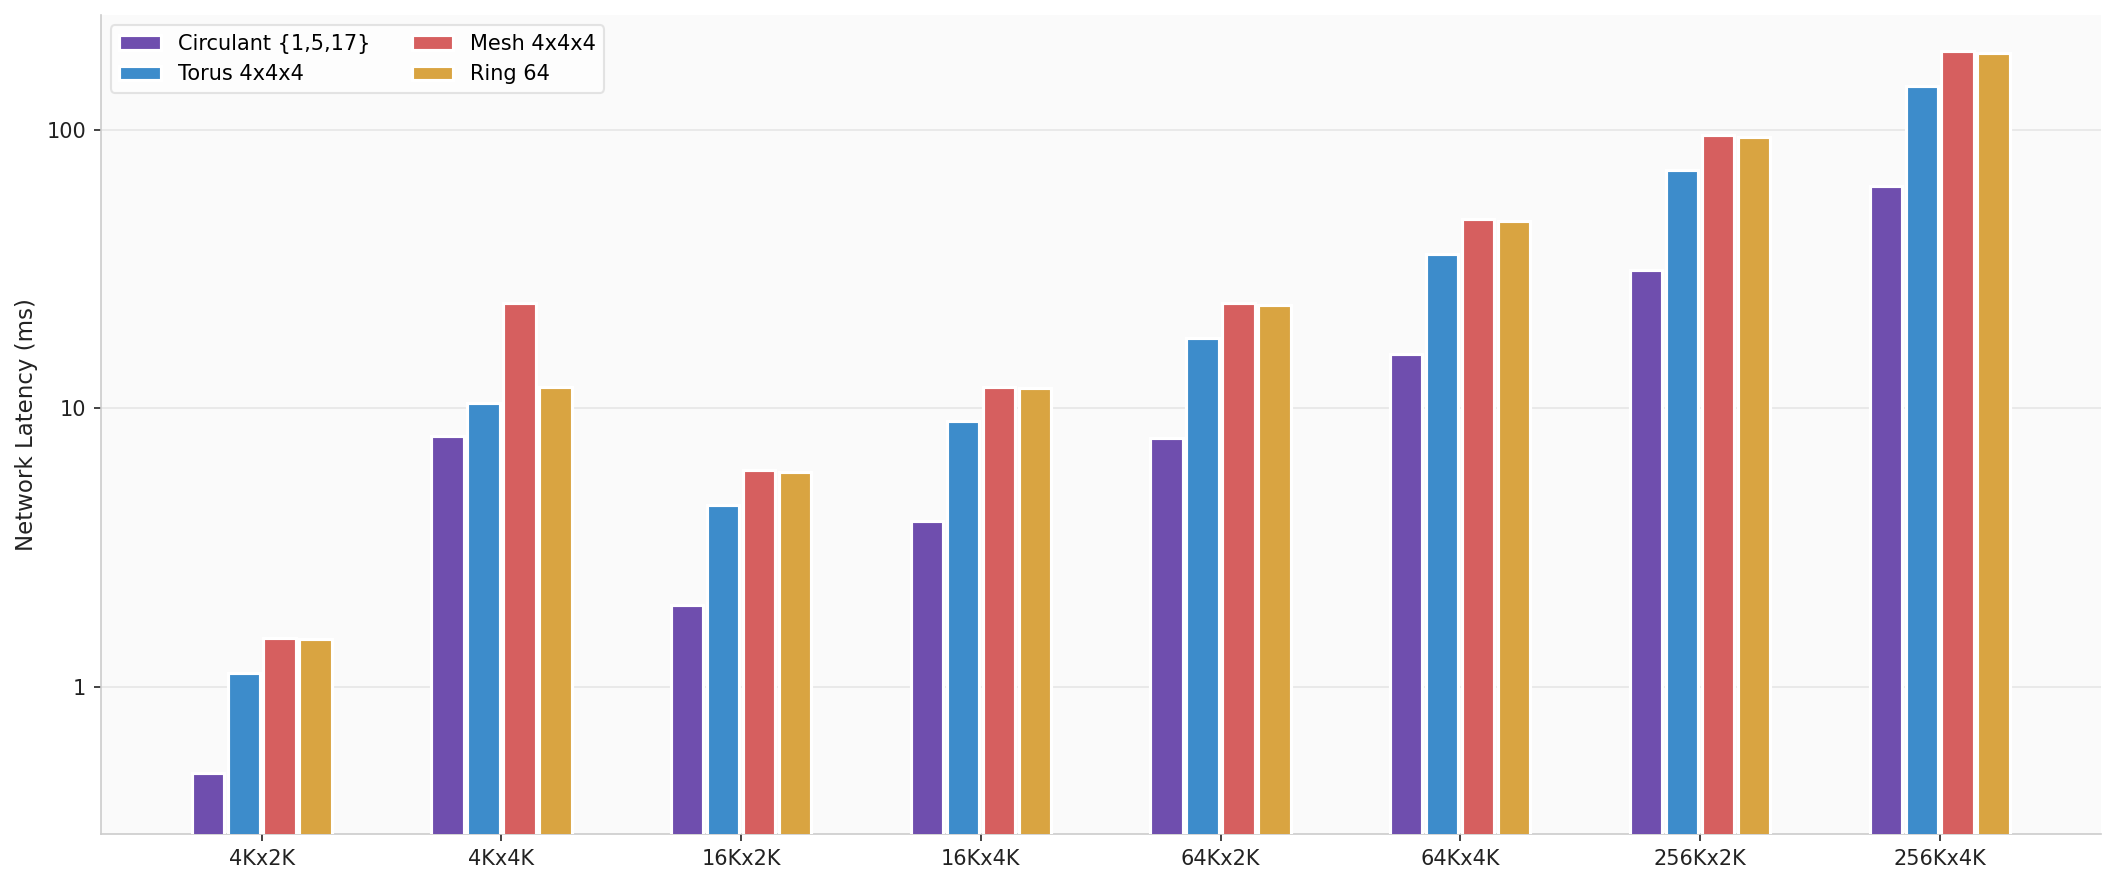
\includegraphics[width=0.92\textwidth]{square_latency_comparison.png}
\caption{Network latency for the square matmul workloads. Each bar group
represents an $N\times N$ by $N\times T$ product; the circulant graph wins all
eight cases and averages $2.16\times$ lower latency than the torus. The
y-axis uses a log scale so both small and large workloads remain visible.}
\label{fig:square-latency}
\end{figure*}

Figure~\ref{fig:square-latency} shows the square matmul results. The
circulant graph averages $3.04\times$ lower latency than the worst topology in
each workload block. On the largest $256\mathrm{K}\times4\mathrm{K}$ case, the
network-only latency is 62.6 ms on the circulant, 143.2 ms on the torus,
190.9 ms on the mesh, and 187.9 ms on the ring.

\begin{figure*}[t]
\centering
\begin{minipage}[t]{0.49\textwidth}
\centering
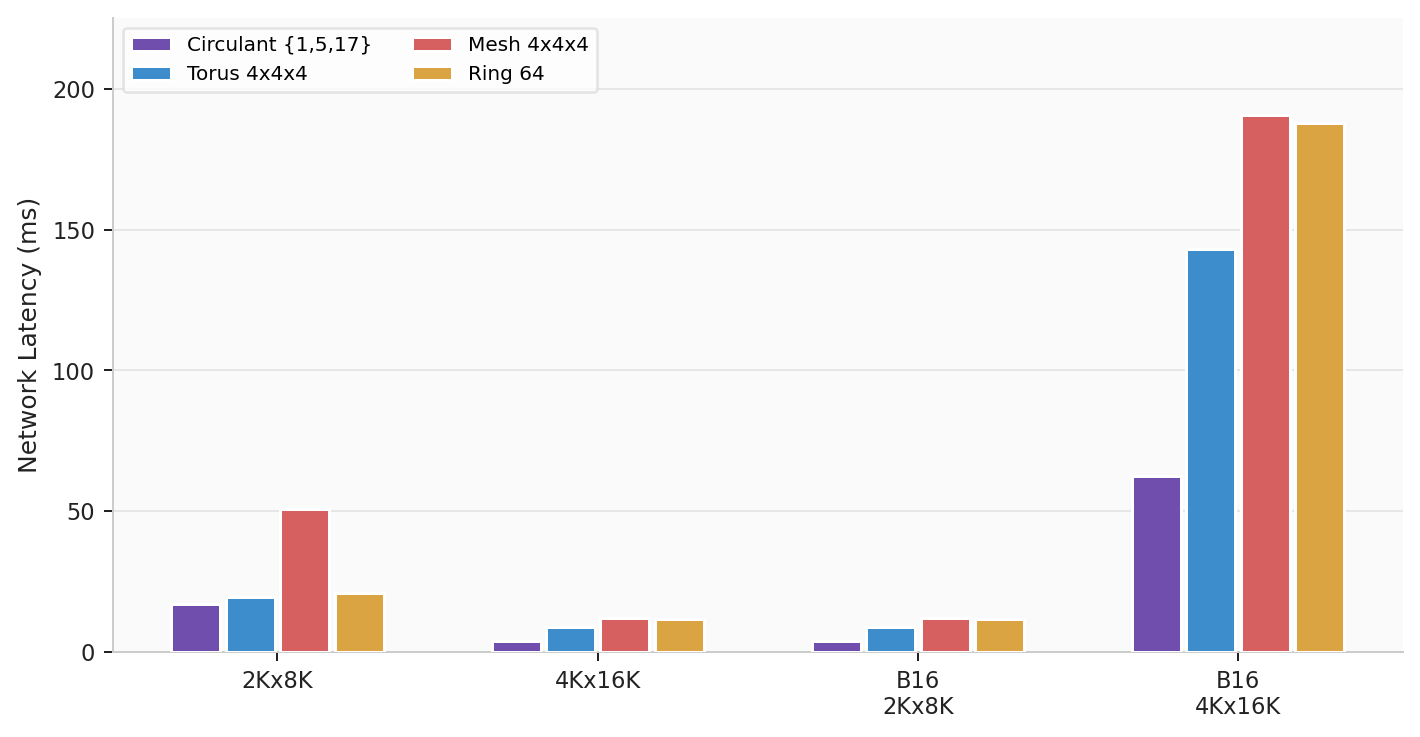
\includegraphics[width=\linewidth]{small_latency_comparison_a.png}\\[-0.5ex]
\footnotesize (a) Batch sizes 1 and 16.
\end{minipage}\hfill
\begin{minipage}[t]{0.49\textwidth}
\centering
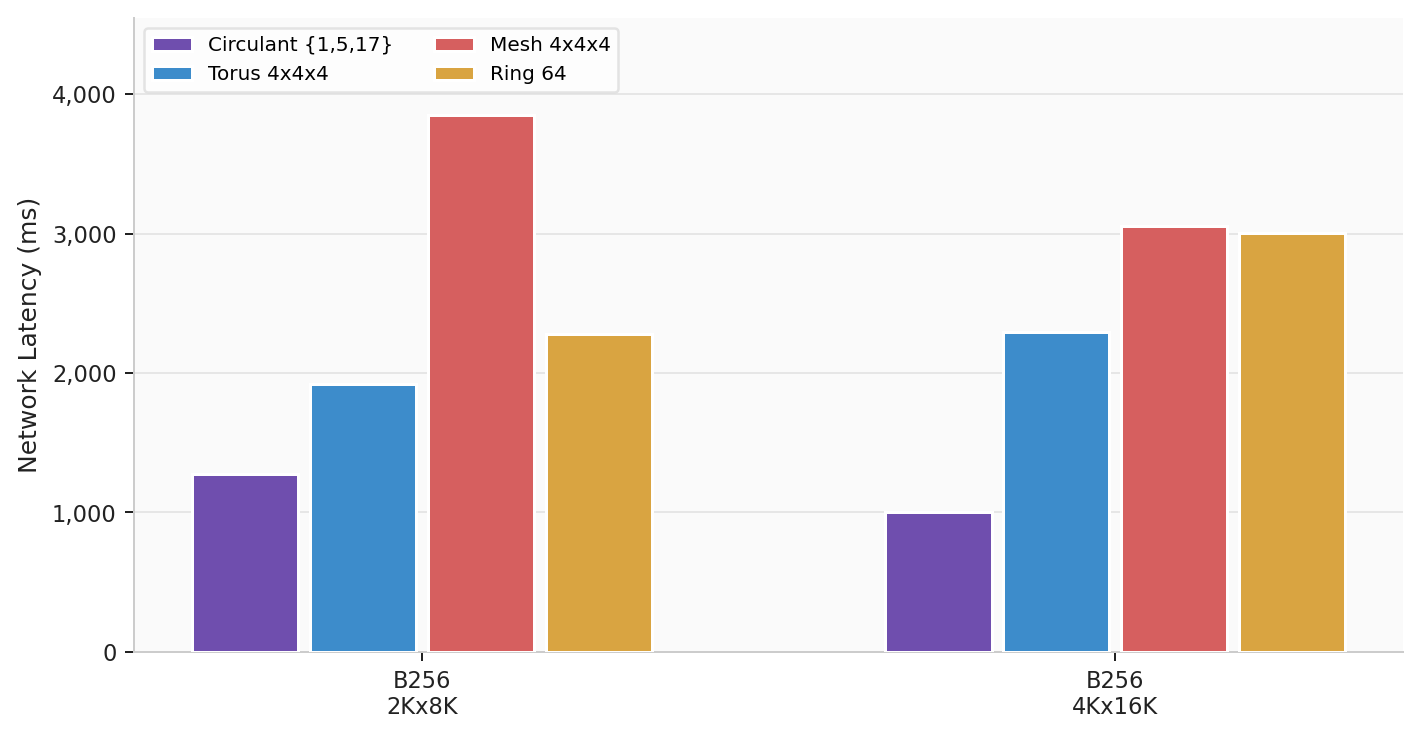
\includegraphics[width=\linewidth]{small_latency_comparison_b.png}\\[-0.5ex]
\footnotesize (b) Batch size 256.
\end{minipage}
\caption{Latency comparison for the small batched matmul workloads. The
two panels use independent y-axes so the smaller batch-size results remain
visible; the circulant graph wins both shapes at batch sizes 1, 16, and 256.}
\label{fig:small-latency}
\end{figure*}

Figure~\ref{fig:small-latency} highlights the small-workload latency comparison.
For example, the $B=256$, $4\mathrm{K}\times16\mathrm{K}$ case takes 1.00 s on
the circulant, 2.29 s on the torus, 3.05 s on the mesh, and 3.01 s on the ring.
The ranking is not caused by total transferred bytes, which are the same across
topologies for a fixed mapping; it comes from how much of that traffic is forced
through the busiest physical link.

\subsection{Latency Breakdown}
The latency breakdown confirms that serialization dominates fixed hop latency.
Across all topology rows, serialization is 99.96\% of modeled network latency
for the small workloads, 99.83\% for the tall workloads, and 99.88\% for the
square workloads. Thus, reducing graph diameter helps, but the main effect is
reducing max-link load. Figure~\ref{fig:tall-lat}
shows the $B=256$ breakdown for the larger tall shapes: the network portion is
roughly half of total modeled latency, so topology remains visible even when
compute is included.

\begin{figure}[!t]
\centering
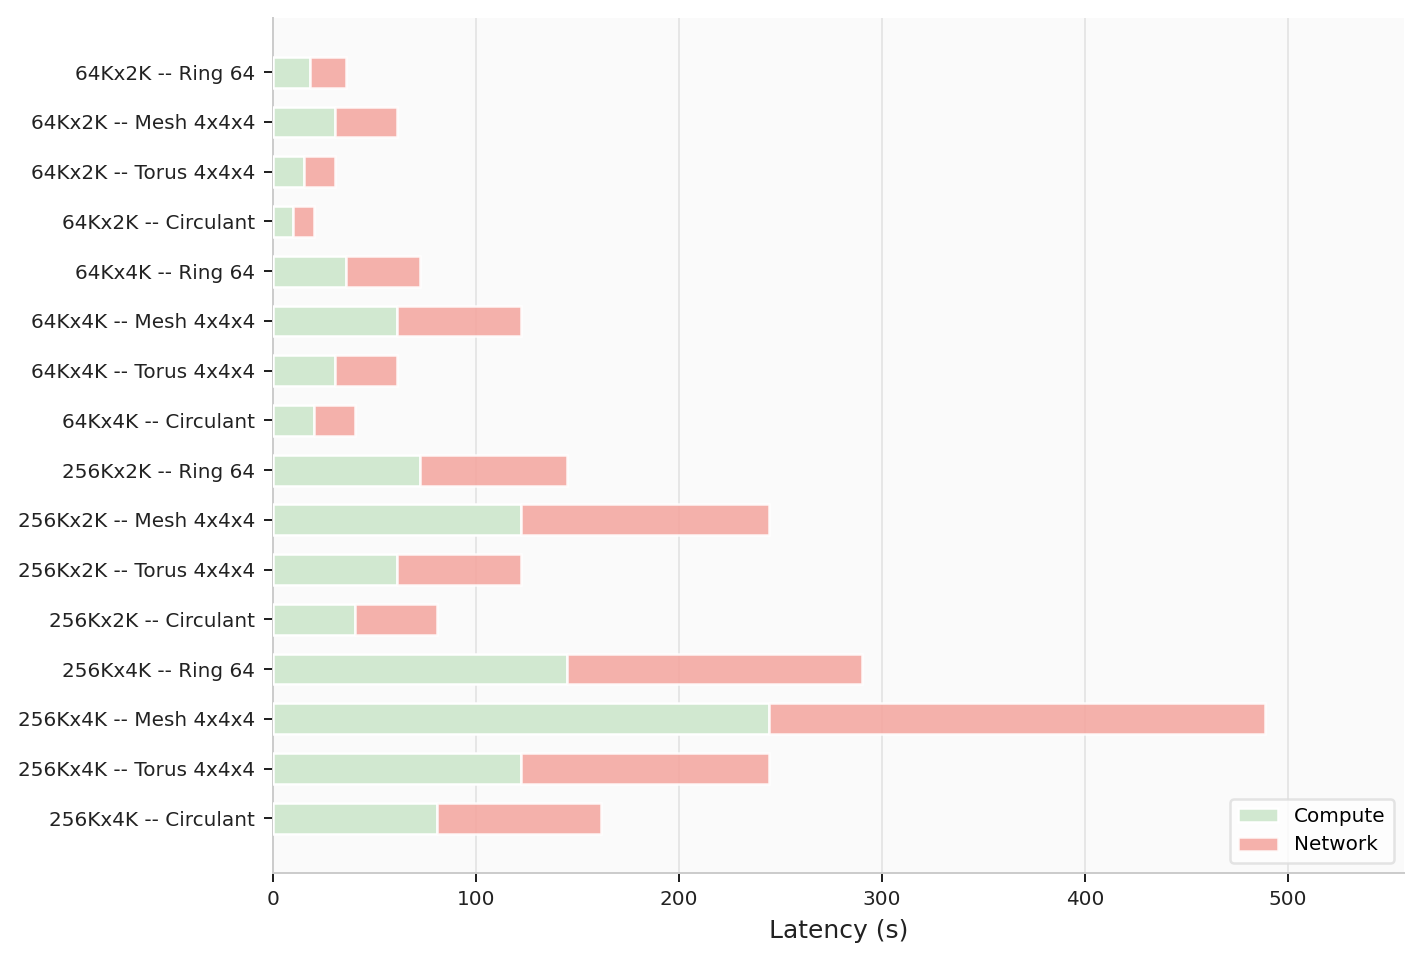
\includegraphics[width=\linewidth]{tall_map64_b256_latency_breakdown_b.png}
\caption{Latency breakdown for $B=256$ tall workloads with
$64\mathrm{K}$ and $256\mathrm{K}$ rows. The network term is large enough for
topology choice to change end-to-end latency, not only network-only latency.}
\label{fig:tall-lat}
\end{figure}

\subsection{Energy Results}
The energy breakdown behaves differently from latency because network energy is
a total bit-hop metric, not a bottleneck-link metric. Figure~\ref{fig:small-en}
shows compute and network energy for the small workloads. Network energy is often
most of the total energy, averaging 88\% across the small topology rows.

\begin{figure}[t]
\centering
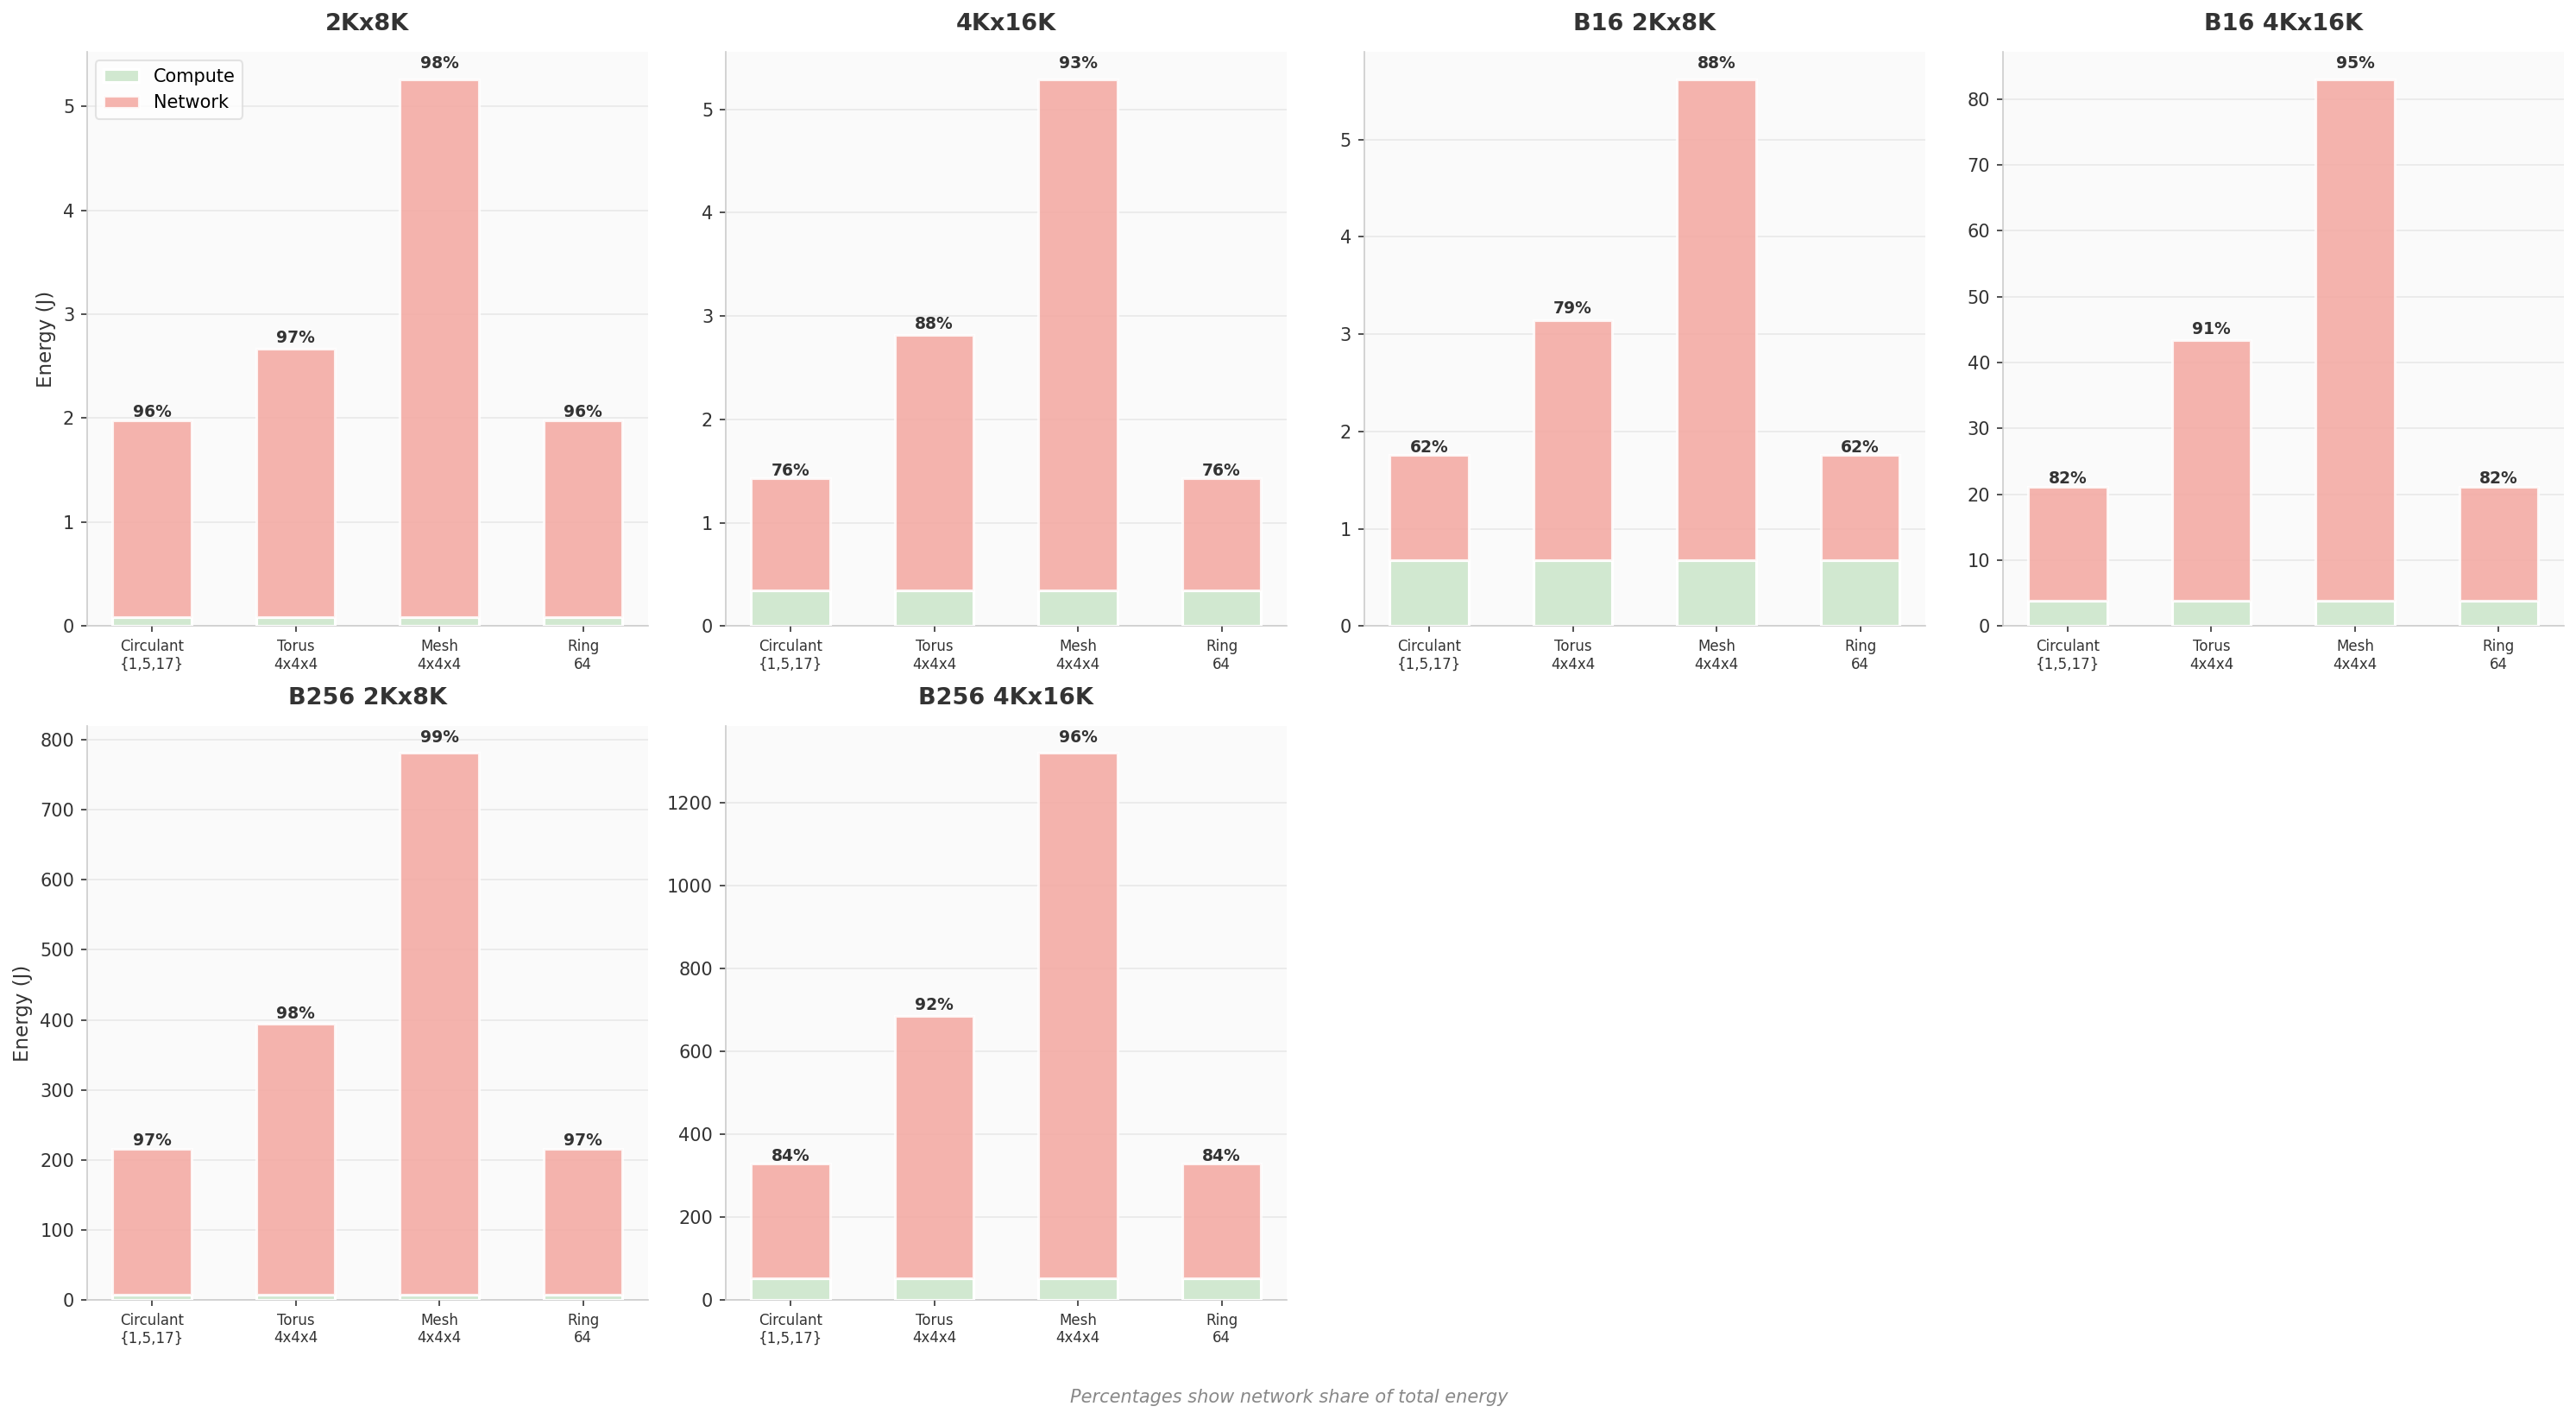
\includegraphics[width=\linewidth]{small_energy_breakdown.png}
\caption{Energy breakdown for the small batched matmul workloads. Network
energy is a large share of total energy even for these small shapes.}
\label{fig:small-en}
\end{figure}

Figure~\ref{fig:tall-en} isolates network energy for the larger $B=256$ tall
workloads. The ring has the same network energy as the circulant because the
model charges one hop per physical link and both schedules have the same total
bit-hop count in these cases, but the ring is slower because two links per chip
create a much higher serialization bottleneck. On average in this plotted
workload group, the torus uses $1.86\times$ and the mesh uses $3.71\times$ the
circulant's network energy. For the largest
$256\mathrm{K}\times4\mathrm{K}$ case, network energy is 13.3 kJ on the
circulant and ring, 24.7 kJ on the torus, and 49.4 kJ on the mesh.

\subsection{MoE Expert-FFN Results}
The MoE expert-FFN experiment uses the same mapper-backed feedback loop as the
matmul experiments. The mapper keeps \texttt{ExpertUp} local and induces one
ReduceScatter on \texttt{ExpertDown:Y}, so the result stresses full-chip
reduction bandwidth rather than sparse token dispatch. Figure~\ref{fig:moe}
shows the network-only latency across token counts. The circulant wins all four
cases, averaging $2.29\times$ lower latency than the torus,
$3.05\times$ lower latency than the mesh, and $3.00\times$ lower latency than
the ring. At $T=4096$, latency is 47.0 ms on the circulant, 107.4 ms on the
torus, 143.2 ms on the mesh, and 140.9 ms on the ring. The near-linear token
scaling follows from the stable ReduceScatter plan and serialization-dominated
traffic.

\begin{figure}[!t]
\centering
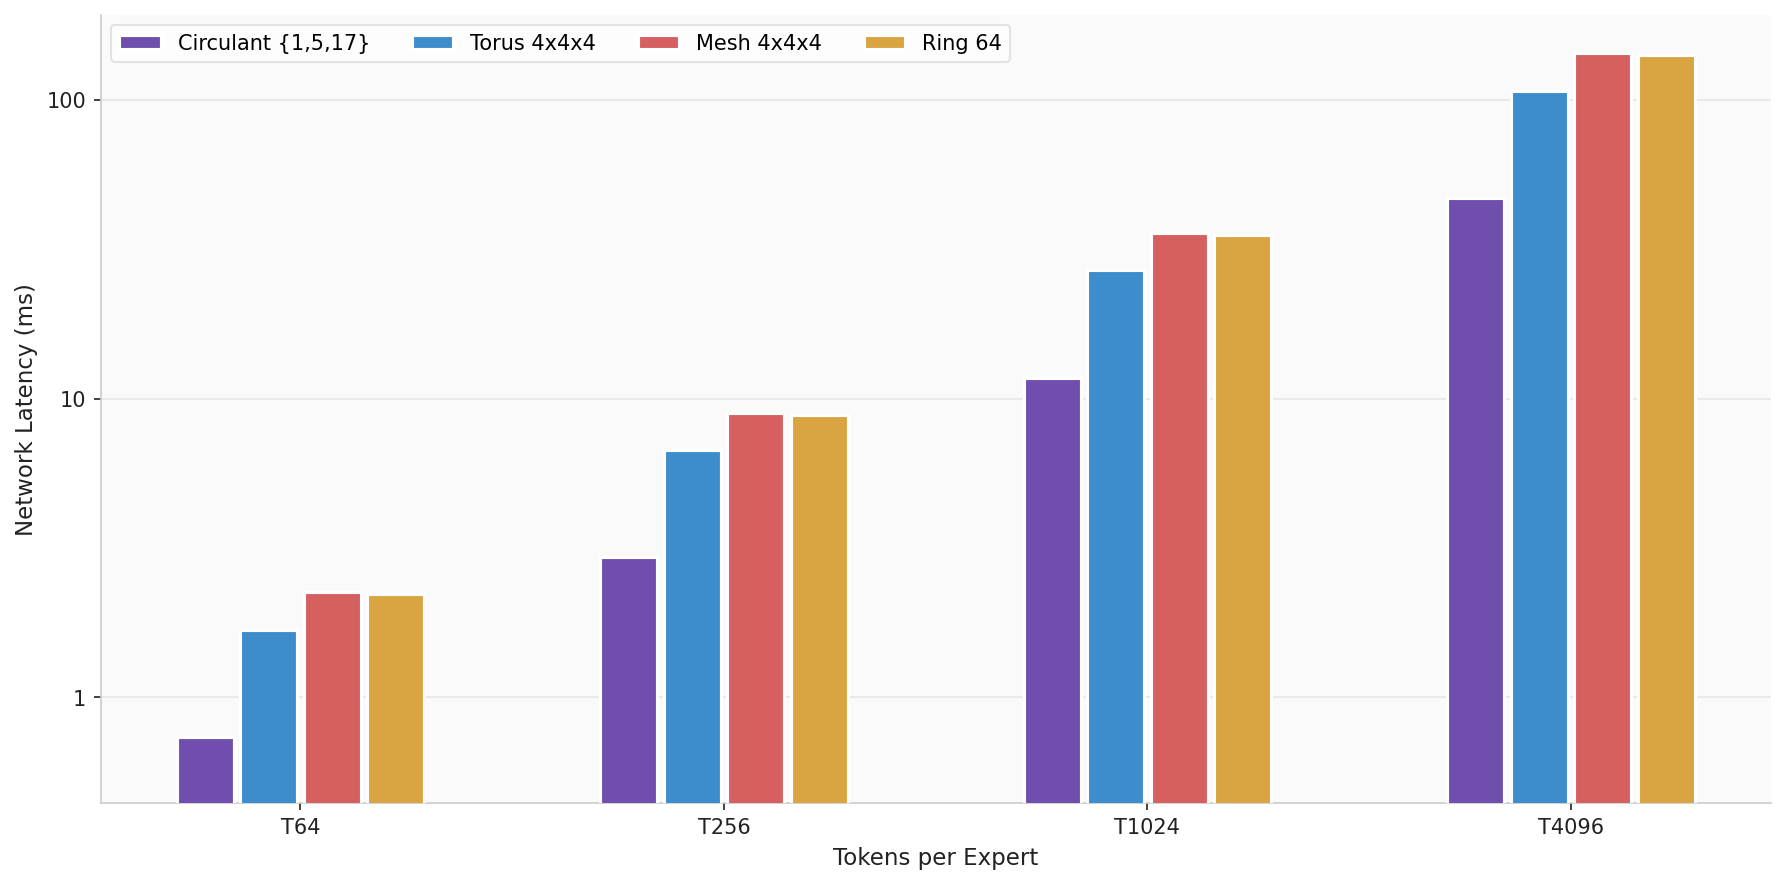
\includegraphics[width=\linewidth]{moe_expert_ffn_latency_comparison.png}
\caption{Network latency for the mapper-backed MoE expert-FFN workloads. The
workload has 16 experts and varies tokens per expert; the y-axis uses a log
scale so the smallest token count remains visible.}
\label{fig:moe}
\end{figure}

\subsection{Mapping Sensitivity}
The feedback-loop results answer the mapping-sensitivity question from the
project prompt. The actual network model substantially increases the estimated
cost relative to the initial proxy model, but the collective plan is stable:
all successful small, tall, square, and MoE expert-FFN runs converge in two
iterations, and the first-to-final inferred collective plan does not change.
Thus, for these workloads, topology mostly changes the cost of a chosen
partitioning rather than causing AccelForge to select a different communication
structure.

\section{Limitations}
The model is useful for controlled topology comparisons, but it is not a full
inference-engine simulator. Full-architecture passes produced implausible
network latencies around 2000 s because our replay serializes coarse inferred
events and omits compute/communication pipelining, kernel fusion,
FlashAttention-style tiling and cache reuse, and serving-runtime scheduling.
Thus, the results should be read as topology studies for extracted collectives
and focused matmul/MoE kernels, not absolute serving predictions. Three
deployment costs are also outside scope: irregular circulant links may be
harder to route physically than a 3D torus, rectangular torus slices are simpler
for allocation and failure handling, and our workloads do not cover Google's
full production traffic mix.

\begin{figure}[!t]
\centering
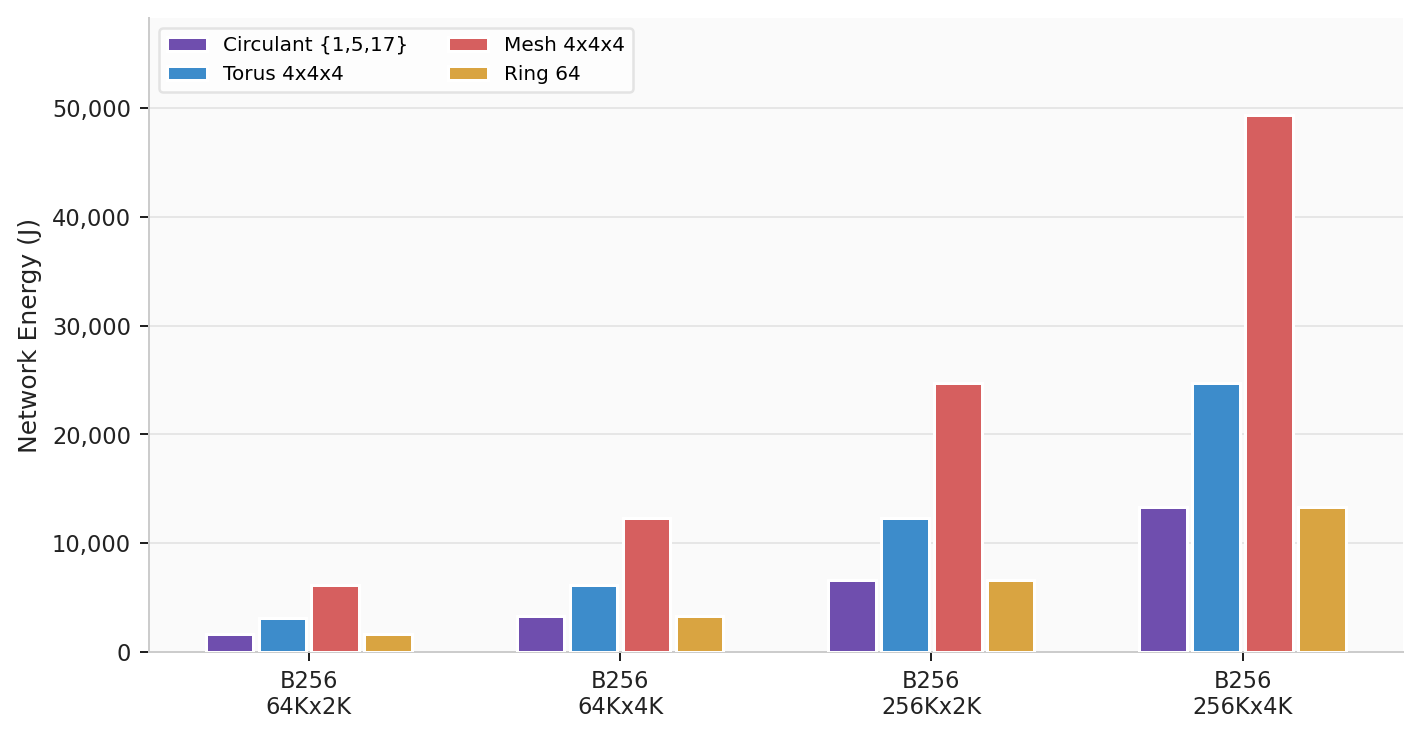
\includegraphics[width=\linewidth]{tall_map64_b256_energy_comparison_b.png}
\caption{Network-energy comparison for $B=256$ tall workloads with
$64\mathrm{K}$ and $256\mathrm{K}$ rows. Energy follows bit-hops, so it does
not always rank topologies the same way as latency.}
\label{fig:tall-en}
\end{figure}

\section{Conclusion}
The experiments support the central claim: under the same six-link-per-chip
budget as a TPU-v4-like 3D torus, a Hamiltonian-decomposable circulant graph is
a better fit for the collective patterns generated by our distributed inference
workloads. Its advantage is not due to adding hardware links; it comes from
spreading large collectives over a lower-diameter, edge-disjoint structure and
reducing the bottleneck-link load. Across the evaluated small, tall, square,
and MoE expert-FFN AccelForge-backed experiments, the circulant wins every
workload, while feedback analysis shows that the mapping stabilizes quickly and
does not change collective structure after network costs are fed back.

\clearpage
% The LLM Usage and References sections do not count toward the page limit.

\section{LLM Usage}
\noindent We used LLMs to format tables and figures for presentation,
aid in the coding process, and revise our language in the report. It was also
helpful for searching for simple information across many JSON results files and
keeping the report organized under the page limit.

\begin{thebibliography}{00}
\bibitem{tpuv4}
N. Jouppi et al., ``TPU v4: An Optically Reconfigurable Supercomputer for
Machine Learning with Hardware Support for Embeddings,'' \emph{ISCA}, 2023.

\bibitem{transformer}
A. Vaswani et al., ``Attention Is All You Need,'' \emph{NeurIPS}, 2017.

\bibitem{megatron}
M. Shoeybi et al., ``Megatron-LM: Training Multi-Billion Parameter Language
Models Using Model Parallelism,'' arXiv:1909.08053, 2019.

\bibitem{gshard}
D. Lepikhin et al., ``GShard: Scaling Giant Models with Conditional
Computation and Automatic Sharding,'' \emph{ICLR}, 2021.

\bibitem{switch}
W. Fedus, B. Zoph, and N. Shazeer, ``Switch Transformers: Scaling to Trillion
Parameter Models with Simple and Efficient Sparsity,'' \emph{JMLR}, 2022.

\bibitem{circulant_survey}
F. K. Hwang, ``A Survey on Multi-Loop Networks,'' \emph{Journal of Research of
the National Bureau of Standards}, vol. 85, no. 4, 1980.
\end{thebibliography}

\end{document}
